\documentclass[14pt,a4paper]{scrartcl}
\usepackage{cmap}
\usepackage[utf8]{inputenc}
\usepackage[T1,T2A]{fontenc}
\usepackage[english,russian]{babel}
\usepackage{relsize}
\usepackage{graphicx}
\usepackage{subfigure}
\usepackage{mathtools}
\usepackage{amssymb}
\usepackage{float}
\usepackage{sidecap}
\usepackage{wrapfig}
\usepackage{caption}
\usepackage[table,xcdraw]{xcolor}
\usepackage{listings}
\usepackage{amsmath,cryptocode}
\usepackage{listings}
\usepackage{booktabs}
\usepackage{multirow}  
\usepackage{multicol}
\usepackage{bigstrut}
\usepackage{lscape}
\usepackage{rotating}
\usepackage{adjustbox}
\usepackage{minted}
\usepackage{breqn}
\usepackage{physics}


\newcommand\scalemath[2]{\scalebox{#1}{\mbox{\ensuremath{\displaystyle #2}}}}


\begin{document}
	\begin{titlepage}
	\begin{center}
		\large
		МИНИСТЕРСТВО ОБРАЗОВАНИЯ И НАУКИ\\ РОССИЙСКОЙ ФЕДЕРАЦИИ
		
		\vspace{0.5cm}
		
		МГТУ им Н.Э.Баумана
		\vspace{0.25cm}
		
		Факультет ФН
		
		Кафедра вычислительной математики и математической физики
		\vfill
		
		
		Соколов Арсений Андреевич\\
		\vfill
		
		
		{\LARGE Домашнее задание №4 по основам сеточных методов \\[2mm]
		}
		\bigskip
		
		3 курс, группа ФН11-63Б\\
		Вариант 3
	\end{center}
	\vfill
	
	\newlength{\ML}
	\settowidth{\ML}{«\underline{\hspace{0.7cm}}» \underline{\hspace{2cm}}}
	\hfill\begin{minipage}{0.4\textwidth}
		Преподаватель\\
		\underline{\hspace{3cm}} В.\,А.~Кутыркин\\
		«\underline{\hspace{0.7cm}}» \underline{\hspace{1.71cm}} 2020 г.
	\end{minipage}%
	\bigskip
	
	
	\vfill
	
	\begin{center}
		Москва, 2020 г.
	\end{center}
\end{titlepage}

\section*{Задание}
\textbf{Задание.}\\

Используя конечные разностные явную и неявную схемы, индуцированные двумерной равномерной сеткой на квадрате $[0;1]\times[0;1]$ с шагом $h = \tau = 0.025$ найти численное решение задачи Коши для одномерного параболического уравнения:

\begin{equation}\label{1}
\left\{\begin{array}{l}
\frac{\partial \varphi(t, x)}{\partial t}-\frac{\partial^{2} \varphi(t, x)}{\partial x^{2}}=-2 \beta+\frac{\alpha \beta \pi\left(x-x^{2}\right)}{2}\cos(\frac{\pi}{2}t) - 2\alpha\beta\sin(\frac{\pi}{2}t), \quad (t,x) \in (0;1)\times(0;1); \\
\varphi(0, x)=2 \beta, x \in[0 ; 1] \quad \textup{(начальное условие)};\\
\varphi(t, 0)=2 \beta(1-t)=\varphi(t, 1), t \in[0 ; 1]  \quad \textup{(краевые условия)};\\
\beta=\frac{N}{2}, \alpha=\frac{1}{64-n}.
\end{array}\right.
\end{equation}


При решении СЛАУ в неявной схеме использовать метод <<прогонки>>. Оценить абсолютные погрешности численных решений. Графически продемонстрировать аналитические и численные решения для моментов времени $t = 0.5$ и $t = 1$ (отдельно для явной схемы, отдельно для неявной схемы). Получившиеся результаты прокомментировать в выводах.

\pagebreak

\section*{Решение} 

Для начала сразу заметим, что, используя данные из условия, не получится достигнуть условия аппроксимации схемы аналитического решения, а именно: $\frac{2D\tau}{h^2} < 1, \quad h,\tau \rightarrow 0$. Действительно, $\frac{2 \cdot 1 \cdot 0.025}{0.025^2} = 80 \gg 1$. Поступим следующим образом: изменим начальные данные до $h = 0.05, \quad \tau = 0.001$. Теперь $\frac{2 \cdot 1 \cdot 0.001}{0.05^2} = 0.8$, что дает выполнение условия аппроксимации схемы аналитическое решения.


Подставим начальные данные ($N = 63, n = 3$) в систему (\ref{1}):

\begin{equation*}
	\left\{\begin{array}{l}
	\frac{\partial \varphi(t, x)}{\partial t}-\frac{\partial^{2} \varphi(t, x)}{\partial x^{2}}=-3+\frac{3 \pi\left(x-x^{2}\right)}{2}\cos(\frac{\pi}{2}t) - 3\sin(\frac{\pi}{2}t), \quad (t,x) \in (0;1)\times(0;1); \\
	\varphi(0, x)=3, x \in[0 ; 1] \quad \textup{(начальное условие)};\\
	\varphi(t, 0)=3(1-t)=\varphi(t, 1), t \in[0 ; 1]  \quad \textup{(краевые условия)};\\
	\beta=\frac{3}{2}, \alpha=1.
	\end{array}\right.
\end{equation*}

\subsection*{Аналитическое решение}

Рассмотрим $\varphi(t,x) = u(t,x) + w(t,x)$, где $w(t,x) = a(t)x + b(t)$, причём $w(t,x)$ удовлетворяет граничным условиям. Тогда $w(t,x) = \frac{\varphi(t,1) - \varphi(t,0)}{1}x + \varphi(t,0) = 3-3t$.

Задача относительно $u(t,x)$:

\begin{equation*}
	\left\{\begin{array}{c}
	\frac{\partial \varphi(t, x)}{\partial t}-\frac{\partial^{2} \varphi(t, x)}{\partial x^{2}}=-3+\frac{3 \pi\left(x-x^{2}\right)}{2}\cos(\frac{\pi}{2}t) - 3\sin(\frac{\pi}{2}t) \\
	\varphi(0, x)=0 \\
	\varphi(t, 0)=0 \\
	\varphi(t, 1)=0
	\end{array}\right.
\end{equation*}

Рассмотрим решение в виде $${u(t,x) = \sum\limits_{k=1}^\infty u_k(t,x) = \sum\limits_{k=1}^\infty T_k(t)X_k(x)}$$ и $${f(t,x) = \sum\limits_{k=1}^\infty F_k(t,x) = \sum\limits_{k=1}^\infty f_k(t)X_k(x)}$$. Подставим данные выражения в уравнение для $u$, получим:

\begin{equation*}
	\sum\limits_{k=1}^\infty (T'_k(t) \cdot X_k(x) - T'_k(t)X''_k(x)) = \sum\limits_{k = 1}^\infty f_k(t)\cdot X_k(x)
\end{equation*}

\begin{equation*}
	\sum\limits_{k=1}^\infty \frac{T'_k(t)}{T_k(t)} - \frac{f_k(t)}{T_k(t)} = \sum\limits_{k=1}^\infty \frac{X''_k(t)}{X_k(t)}
\end{equation*}

\begin{equation*}
	X''_k(x) + \lambda_kX_k(x) = 0
\end{equation*}

\begin{equation*}
	T'_k(t) + \lambda_kT_k(t) = f_k(t)
\end{equation*}

\begin{equation*}
	X_k(0) = X_k(1) = 0
\end{equation*}

\begin{equation*}
	T_k(t) = 0
\end{equation*}


Отсюда $X_k(x) = \sin(\pi k x), \quad \lambda_k = \pi^2 k^2$ и 

\begin{equation*}
	T_k(t) = \int_{0}^{t}\mathbf{e}^{-\pi^2k^2(t-\tau)} f_k(\tau)\mathbf{d}\tau = \int_{0}^{t}2\mathbf{e}^{-\pi^2k^2(t-\tau)} \int_{0}^{1}f(\xi,\tau)\sin(k \pi \xi) \mathbf{d}\xi \mathbf{d}\tau
\end{equation*}


Чтобы построить график и сравнить полученное аналитическое решение с численным рассмотрим первые 100 слагаемых бесконечной суммы.

Построим графики:

\begin{figure}[H]
	\begin{minipage}[h]{1\linewidth}
		\center{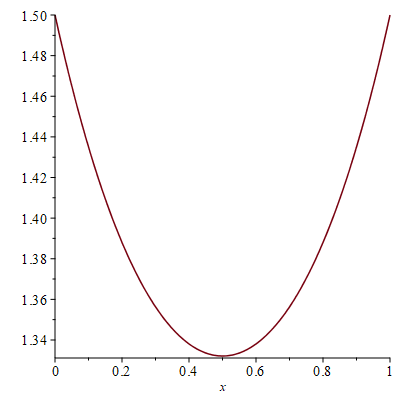
\includegraphics[width=.7\linewidth]{../img/analit_5.png}}\\
		\caption{График аналитического решения при $t=0.5$}
	\end{minipage}
\end{figure}


\begin{figure}[H]
	\begin{minipage}[h]{1\linewidth}
		\center{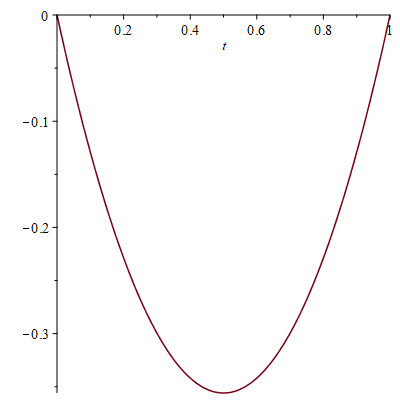
\includegraphics[width=.7\linewidth]{../img/analit_1.png}}\\
		\caption{График аналитического решения при $t=1$}
	\end{minipage}
\end{figure}


\pagebreak
\subsection*{Численное решение. Явная разностная схема}

Явная разностная схема имеет вид:

\begin{figure}[H]
	\begin{minipage}[h]{1\linewidth}
		\center{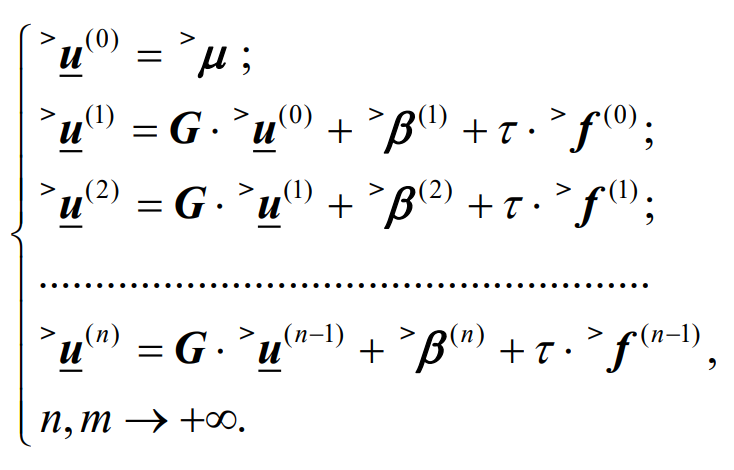
\includegraphics[width=.7\linewidth]{../img/f1.png}}\\
	\end{minipage}
\end{figure}

где использованы обозначения:

\begin{figure}[H]
	\begin{minipage}[h]{1\linewidth}
		\center{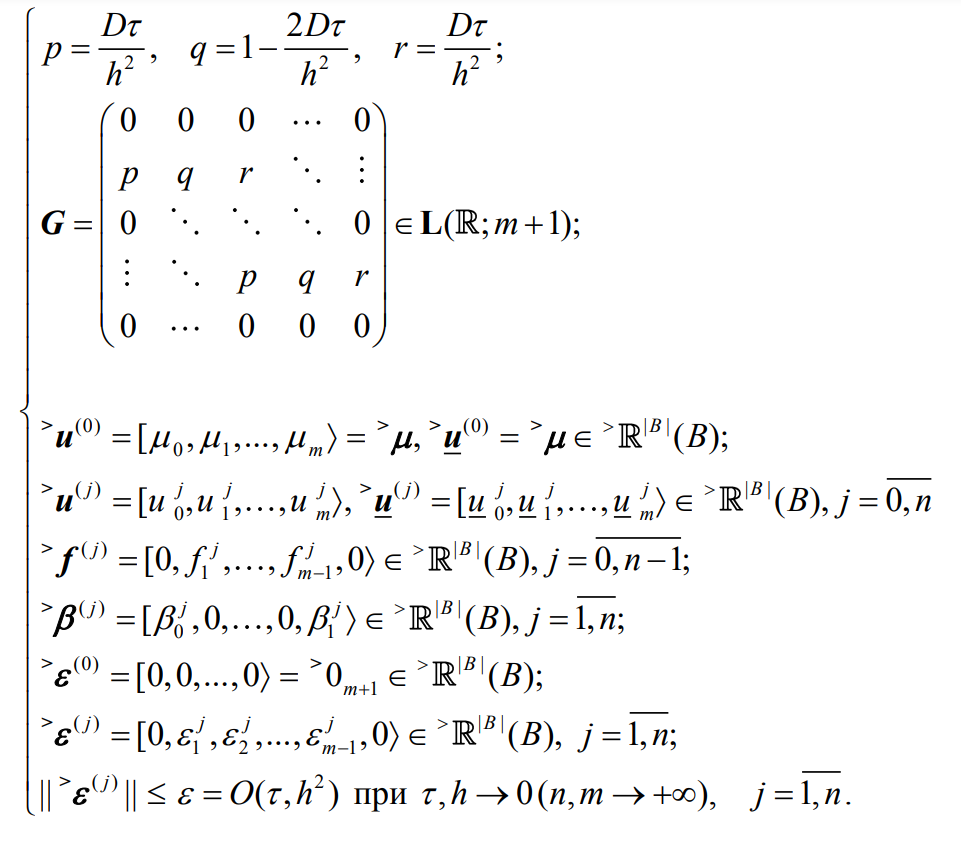
\includegraphics[width=.7\linewidth]{../img/f2.png}}\\
	\end{minipage}
\end{figure}


\begin{equation*}
	u_i^j = u(t_j;x_i), \quad f_i^j = f(t_j;x_i), \quad \mu_i=\mu(x_i), \quad \beta_0^j = \beta_0(t_j), \quad \beta_1^j=\beta_1(t_j)
\end{equation*}

\pagebreak
Тогда матрица $\mathbf{G}$ примет вид:

\resizebox{\linewidth}{!}{%
\begin{equation*}
	G = \left[ \begin {array}{ccccccccccccccccccccc}  0& 0& 0& 0& 0
	& 0& 0& 0& 0& 0& 0& 0& 0& 0& 0& 0& 0& 0& 0
	& 0& 0\\ \noalign{\medskip} 0.4& 0.2& 0.4& 0& 0& 0& 0& 0
	& 0& 0& 0& 0& 0& 0& 0& 0& 0& 0& 0& 0& 0
	\\ \noalign{\medskip} 0& 0.4& 0.2& 0.4& 0& 0& 0& 0& 0& 0
	& 0& 0& 0& 0& 0& 0& 0& 0& 0& 0& 0
	\\ \noalign{\medskip} 0& 0& 0.4& 0.2& 0.4& 0& 0& 0& 0& 0
	& 0& 0& 0& 0& 0& 0& 0& 0& 0& 0& 0
	\\ \noalign{\medskip} 0& 0& 0& 0.4& 0.2& 0.4& 0& 0& 0& 0
	& 0& 0& 0& 0& 0& 0& 0& 0& 0& 0& 0
	\\ \noalign{\medskip} 0& 0& 0& 0& 0.4& 0.2& 0.4& 0& 0& 0
	& 0& 0& 0& 0& 0& 0& 0& 0& 0& 0& 0
	\\ \noalign{\medskip} 0& 0& 0& 0& 0& 0.4& 0.2& 0.4& 0& 0
	& 0& 0& 0& 0& 0& 0& 0& 0& 0& 0& 0
	\\ \noalign{\medskip} 0& 0& 0& 0& 0& 0& 0.4& 0.2& 0.4& 0
	& 0& 0& 0& 0& 0& 0& 0& 0& 0& 0& 0
	\\ \noalign{\medskip} 0& 0& 0& 0& 0& 0& 0& 0.4& 0.2& 0.4
	& 0& 0& 0& 0& 0& 0& 0& 0& 0& 0& 0
	\\ \noalign{\medskip} 0& 0& 0& 0& 0& 0& 0& 0& 0.4& 0.2
	& 0.4& 0& 0& 0& 0& 0& 0& 0& 0& 0& 0
	\\ \noalign{\medskip} 0& 0& 0& 0& 0& 0& 0& 0& 0& 0.4
	& 0.2& 0.4& 0& 0& 0& 0& 0& 0& 0& 0& 0
	\\ \noalign{\medskip} 0& 0& 0& 0& 0& 0& 0& 0& 0& 0
	& 0.4& 0.2& 0.4& 0& 0& 0& 0& 0& 0& 0& 0
	\\ \noalign{\medskip} 0& 0& 0& 0& 0& 0& 0& 0& 0& 0
	& 0& 0.4& 0.2& 0.4& 0& 0& 0& 0& 0& 0& 0
	\\ \noalign{\medskip} 0& 0& 0& 0& 0& 0& 0& 0& 0& 0
	& 0& 0& 0.4& 0.2& 0.4& 0& 0& 0& 0& 0& 0
	\\ \noalign{\medskip} 0& 0& 0& 0& 0& 0& 0& 0& 0& 0
	& 0& 0& 0& 0.4& 0.2& 0.4& 0& 0& 0& 0& 0
	\\ \noalign{\medskip} 0& 0& 0& 0& 0& 0& 0& 0& 0& 0
	& 0& 0& 0& 0& 0.4& 0.2& 0.4& 0& 0& 0& 0
	\\ \noalign{\medskip} 0& 0& 0& 0& 0& 0& 0& 0& 0& 0
	& 0& 0& 0& 0& 0& 0.4& 0.2& 0.4& 0& 0& 0
	\\ \noalign{\medskip} 0& 0& 0& 0& 0& 0& 0& 0& 0& 0
	& 0& 0& 0& 0& 0& 0& 0.4& 0.2& 0.4& 0& 0
	\\ \noalign{\medskip} 0& 0& 0& 0& 0& 0& 0& 0& 0& 0
	& 0& 0& 0& 0& 0& 0& 0& 0.4& 0.2& 0.4& 0
	\\ \noalign{\medskip} 0& 0& 0& 0& 0& 0& 0& 0& 0& 0
	& 0& 0& 0& 0& 0& 0& 0& 0& 0.4& 0.2& 0.4
	\\ \noalign{\medskip} 0& 0& 0& 0& 0& 0& 0& 0& 0& 0
	& 0& 0& 0& 0& 0& 0& 0& 0& 0& 0& 0\end {array}
	\right] 
\end{equation*}}

\pagebreak

Графики численного решения по явной схеме: 


\begin{figure}[H]
	\begin{minipage}[h]{1\linewidth}
		\center{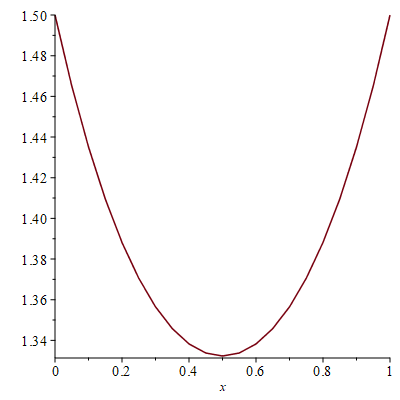
\includegraphics[width=.7\linewidth]{../img/yavn_5.png}}\\
		\caption{График численного явного решения при $t=0.5$}
	\end{minipage}
\end{figure}

Точки:
\begin{align*}
	[[0., 1.50000000000000], [0.5e-1, 1.46512014427974], [.10, 1.43510655875561],\\
	 [.15, 1.40956508234055], [.20, 1.38814550245223], [.25, 1.37054248702328], \\
	 [.30, 1.35649637688430], [.35, 1.34579384496598], [.40, 1.33826842788662], \\
	 [.45, 1.33380093453720], [.50, 1.33231973530111], [.55, 1.33380093453719], \\
	 [.60, 1.33826842788662], [.65, 1.34579384496598], [.70, 1.35649637688430], \\
	 [.75, 1.37054248702328], [.80, 1.38814550245223], [.85, 1.40956508234055], \\
	 [.90, 1.43510655875561], [.95, 1.46512014427974], [1.00, 1.50000000000000]]
\end{align*}

\pagebreak

\begin{figure}[H]
	\begin{minipage}[h]{1\linewidth}
		\center{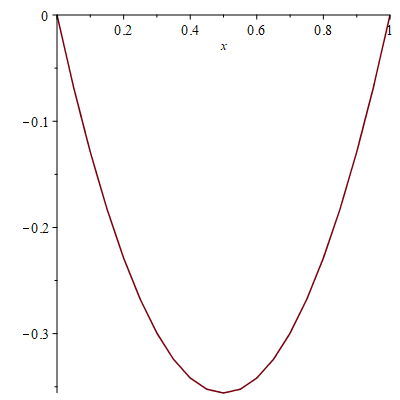
\includegraphics[width=.7\linewidth]{../img/yavn_1.png}}\\
		\caption{График численного явного решения при $t=1$}
	\end{minipage}
\end{figure}

Точки:
\begin{align*}
[[0., 0.], [0.5e-1, -0.682498782974187e-1], [.10, -.129074568429754],\\
 [.15, -.182546754227427], [.20, -.228735070545019], [.25, -.267702411330733],\\
  [.30, -.299504465671840], [.35, -.324188480850184], [.40, -.341792251540464], \\
  [.45, -.352343334412606], [.50, -.355858487578648], [.55, -.352343334412606],\\
   [.60, -.341792251540464], [.65, -.324188480850184], [.70, -.299504465671840], \\
   [.75, -.267702411330733], [.80, -.228735070545019], [.85, -.182546754227427],\\
    [.90, -.129074568429754], [.95, -0.682498782974187e-1], [1.00, 0.]]
\end{align*}



Абсолютная погрешность численного решения явной разностной схемы: $$0.0003313756673828$$

\pagebreak
\subsection*{Численное решение. Неявная разностная схема}

Неявная разностная схема имеет вид:

\begin{figure}[H]
	\begin{minipage}[h]{1\linewidth}
		\center{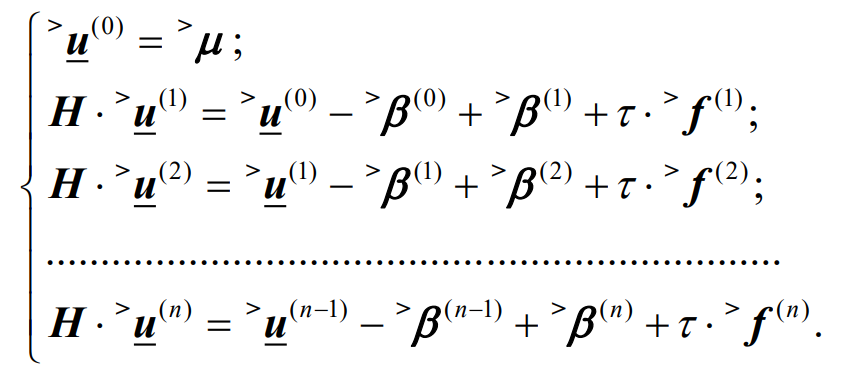
\includegraphics[width=.7\linewidth]{../img/f3.png}}\\
	\end{minipage}
\end{figure}

где использованы обозначения:

\begin{figure}[H]
	\begin{minipage}[h]{1\linewidth}
		\center{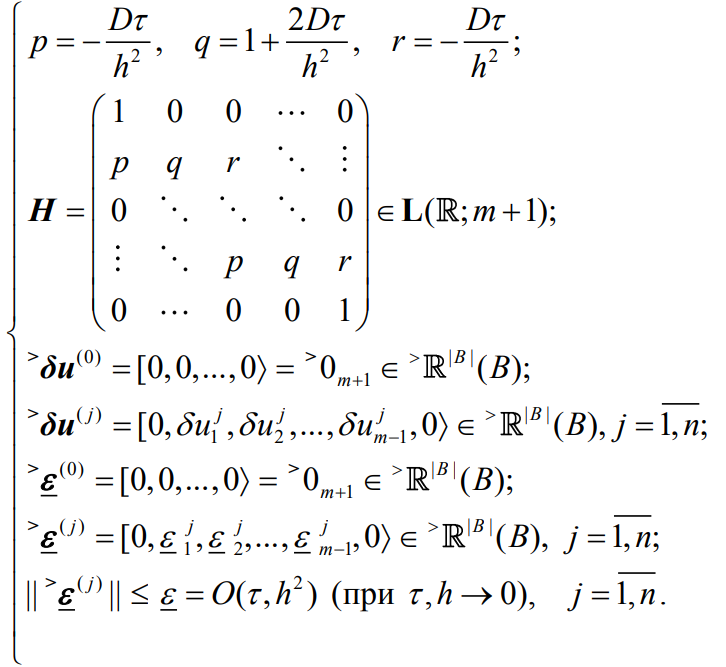
\includegraphics[width=.7\linewidth]{../img/f4.png}}\\
	\end{minipage}
\end{figure}

\pagebreak
Тогда матрица $\mathbf{H}$ примет вид:


\resizebox{\linewidth}{!}{%
	\begin{equation*}
	 H =\left[ \begin {array}{ccccccccccccccccccccc}  1.0& 0& 0& 0& 0
	& 0& 0& 0& 0& 0& 0& 0& 0& 0& 0& 0& 0& 0& 0
	& 0& 0\\ \noalign{\medskip}- 0.4& 2.0&- 0.4& 0& 0& 0& 0&
	0& 0& 0& 0& 0& 0& 0& 0& 0& 0& 0& 0& 0& 0
	\\ \noalign{\medskip} 0&- 0.4& 2.0&- 0.4& 0& 0& 0& 0& 0&
	0& 0& 0& 0& 0& 0& 0& 0& 0& 0& 0& 0
	\\ \noalign{\medskip} 0& 0&- 0.4& 2.0&- 0.4& 0& 0& 0& 0&
	0& 0& 0& 0& 0& 0& 0& 0& 0& 0& 0& 0
	\\ \noalign{\medskip} 0& 0& 0&- 0.4& 2.0&- 0.4& 0& 0& 0&
	0& 0& 0& 0& 0& 0& 0& 0& 0& 0& 0& 0
	\\ \noalign{\medskip} 0& 0& 0& 0&- 0.4& 2.0&- 0.4& 0& 0&
	0& 0& 0& 0& 0& 0& 0& 0& 0& 0& 0& 0
	\\ \noalign{\medskip} 0& 0& 0& 0& 0&- 0.4& 2.0&- 0.4& 0&
	0& 0& 0& 0& 0& 0& 0& 0& 0& 0& 0& 0
	\\ \noalign{\medskip} 0& 0& 0& 0& 0& 0&- 0.4& 2.0&- 0.4&
	0& 0& 0& 0& 0& 0& 0& 0& 0& 0& 0& 0
	\\ \noalign{\medskip} 0& 0& 0& 0& 0& 0& 0&- 0.4& 2.0&-
	0.4& 0& 0& 0& 0& 0& 0& 0& 0& 0& 0& 0
	\\ \noalign{\medskip} 0& 0& 0& 0& 0& 0& 0& 0&- 0.4&
	2.0&- 0.4& 0& 0& 0& 0& 0& 0& 0& 0& 0& 0
	\\ \noalign{\medskip} 0& 0& 0& 0& 0& 0& 0& 0& 0&-
	0.4& 2.0&- 0.4& 0& 0& 0& 0& 0& 0& 0& 0& 0
	\\ \noalign{\medskip} 0& 0& 0& 0& 0& 0& 0& 0& 0& 0
	&- 0.4& 2.0&- 0.4& 0& 0& 0& 0& 0& 0& 0& 0
	\\ \noalign{\medskip} 0& 0& 0& 0& 0& 0& 0& 0& 0& 0
	& 0&- 0.4& 2.0&- 0.4& 0& 0& 0& 0& 0& 0& 0
	\\ \noalign{\medskip} 0& 0& 0& 0& 0& 0& 0& 0& 0& 0
	& 0& 0&- 0.4& 2.0&- 0.4& 0& 0& 0& 0& 0& 0
	\\ \noalign{\medskip} 0& 0& 0& 0& 0& 0& 0& 0& 0& 0
	& 0& 0& 0&- 0.4& 2.0&- 0.4& 0& 0& 0& 0& 0
	\\ \noalign{\medskip} 0& 0& 0& 0& 0& 0& 0& 0& 0& 0
	& 0& 0& 0& 0&- 0.4& 2.0&- 0.4& 0& 0& 0& 0
	\\ \noalign{\medskip} 0& 0& 0& 0& 0& 0& 0& 0& 0& 0
	& 0& 0& 0& 0& 0&- 0.4& 2.0&- 0.4& 0& 0& 0
	\\ \noalign{\medskip} 0& 0& 0& 0& 0& 0& 0& 0& 0& 0
	& 0& 0& 0& 0& 0& 0&- 0.4& 2.0&- 0.4& 0& 0
	\\ \noalign{\medskip} 0& 0& 0& 0& 0& 0& 0& 0& 0& 0
	& 0& 0& 0& 0& 0& 0& 0&- 0.4& 2.0&- 0.4& 0
	\\ \noalign{\medskip} 0& 0& 0& 0& 0& 0& 0& 0& 0& 0
	& 0& 0& 0& 0& 0& 0& 0& 0&- 0.4& 2.0&- 0.4
	\\ \noalign{\medskip} 0& 0& 0& 0& 0& 0& 0& 0& 0& 0
	& 0& 0& 0& 0& 0& 0& 0& 0& 0& 0& 1.0\end {array}
	\right] 
	\end{equation*}}



%%%%%%%%%%%%%%%%%%%%%%%%%%%%%%%%%%%%%%%%%%%%%%%%%%%%%%%%%%%%%%%%%%%%%%%%%%%%%%%%%%%%%%%%%%%%%%
%%%%%%%%%%%%%%%%%%%%%%%%%%%%%%%%%%%%%%%%%%%%%%%%%%%%%%%%%%%%%%%%%%%%%%%%%%%%%%%%%%%%%%%%%%%%%%
%%%%%%%%%%%%%%%%%%%%%%%%%%%%%%%%%%%%%%%%%%%%%%%%%%%%%%%%%%%%%%%%%%%%%%%%%%%%%%%%%%%%%%%%%%%%%%


\pagebreak

Графики численного решения по неявной схеме: 


\begin{figure}[H]
	\begin{minipage}[h]{1\linewidth}
		\center{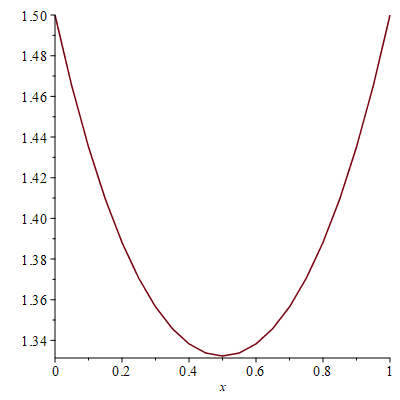
\includegraphics[width=.7\linewidth]{../img/nyavn_5.png}}\\
		\caption{График численного неявного решения при $t=0.5$}
	\end{minipage}
\end{figure}

Точки:
\begin{align*}
[[0., 1.50000000000000], [0.5e-1, 1.46511828754889], [.10, 1.43510284991246],\\
 [.15, 1.40955955422417], [.20, 1.38813823239132], [.25, 1.37053360884059],\\
  [.30, 1.35648608125871], [.35, 1.34578237854569], [.40, 1.33825608599867],\\
   [.45, 1.33378805052480], [.50, 1.33230666634649], [.55, 1.33378804582714],\\
    [.60, 1.33825607663055], [.65, 1.34578236496297], [.70, 1.35648606474227],\\
     [.75, 1.37053359110446], [.80, 1.38813821556771], [.85, 1.40955953917702],\\
      [.90, 1.43510283892470], [.95, 1.46511828181135], [1.00, 1.50000000000000]]
\end{align*}

\pagebreak

\begin{figure}[H]
	\begin{minipage}[h]{1\linewidth}
		\center{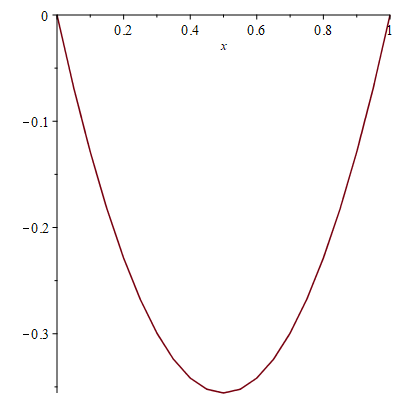
\includegraphics[width=.7\linewidth]{../img/nyavn_1.png}}\\
		\caption{График численного неявного решения при $t=1$}
	\end{minipage}
\end{figure}

Точки:
\begin{align*}
[[0., 0.], [0.5e-1, -0.682364359217568e-1], [.10, -.129048075377762],\\
 [.15, -.182507948748947], [.20, -.228684993436692], [.25, -.267642363435463],\\
  [.30, -.299435965635561], [.35, -.324113224489577], [.40, -.341712071696780],\\
   [.45, -.352260161487117], [.50, -.355774310310583], [.55, -.352260160919589], \\
   [.60, -.341712070536377], [.65, -.324113222788131], [.70, -.299435963606849],\\
    [.75, -.267642361352541], [.80, -.228684991603023], [.85, -.182507947202775],\\ 
    [.90, -.129048074320734], [.95, -0.682364354011660e-1], [1.00, 0.]]
\end{align*}



Абсолютная погрешность численного решения неявной разностной схемы: $$0.0002759265358915$$



\pagebreak

Построим совмещенные графики полученных решений.

\begin{figure}[H]
	\begin{minipage}[h]{1\linewidth}
		\center{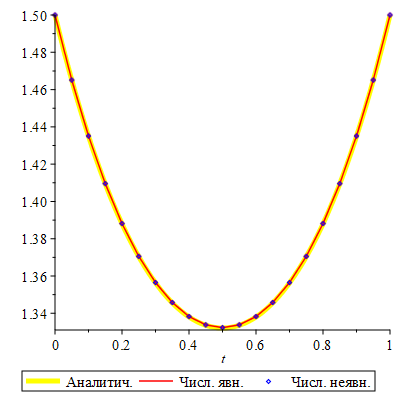
\includegraphics[width=.7\linewidth]{../img/sovm_5.png}}\\
		\caption{Совмещённые графики при $t=0.5$}
	\end{minipage}
\end{figure}

\begin{figure}[H]
	\begin{minipage}[h]{1\linewidth}
		\center{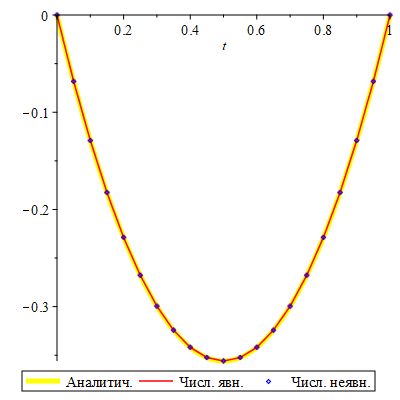
\includegraphics[width=.7\linewidth]{../img/sovm_1.png}}\\
		\caption{Совмещённые графики при $t=1$}
	\end{minipage}
\end{figure}

\textbf{Вывод.} Проанализировав совмещённые графики, можно сделать вывод о том, что аналитическое, численное явное и численное неявное решения хорошо наложились друг на друга. Таким образом, разобранные конечноразностные схемы имеют достаточно высокую точность. Кроме того, нужно еще раз подчеркнуть о важности выполнения условия аппроксимации схемы аналитического решения, а именно: $\frac{2D\tau}{h^2} < 1, \quad h,\tau \rightarrow 0$


\end{document}